\section{Experiment 4. 03.03.2020}\label{experiment-4.-03.03.2020}

It took place on 03.03.2020. The weather condition was appropriate for running experiments, despite that it was raining lightly.

For the fourth attempt, we implement message sending only via HTTP. The main aim of the experiment is to try to place the UEs in three cases (sub-optimal, uniform, near-optimal). Phones forced to push their channel quality metric to the server for each case. On the server-side, GPS\_Tracker tries to find optimal positions for UAVs supposing there are 2 AP is required.

We decided to reduce the area layout to 25x25 meters.

\subsection{Results}\label{results}

The HTTP protocol helps us to receive messages more reliable, although there was a problem, e.g. the further UE is located from AP, the less is probable the reception of the message.

Tests showed reliability of HTTP protocol, therefore, we decided to continue our experiment.

We found out that network speed measurements were not significant, because there was markedly seen difference between uplink and downlink speed, uplink tests threw the timeout exception in case of larger distance between a UE and used AP, since the communication took longer and the session finished.

The measurements showed the following coordinates for the 6 UEs:

\begin{longtable}[]{@{}ll@{}}
\caption{Initial positions for UEs}\tabularnewline
\toprule
Unique ID & Coordinates\tabularnewline
\midrule
\endfirsthead
\toprule
Unique ID & Coordinates\tabularnewline
\midrule
\endhead
f072f812f48ce468 & (50.4056203, 10.5626057)\tabularnewline
eb0b54819c69cf0c & (50.4056230, 10.5626126)\tabularnewline
27349a2cde6592df & (50.4056445, 10.5625865)\tabularnewline
51336504999bc1ca & (50.40567855, 10.5625238)\tabularnewline
b1c225280d0ed13f & (50.4056924, 10.5624943)\tabularnewline
\bottomrule
\end{longtable}

The experiment is divided into four parts:

\begin{itemize}
\tightlist
\item
  Before 11:05 - suboptimal case
\item
  11:05 - 11:08 - uniform case
\item
  11:08 - 11:12 - near-optimal case
\item
  11:12 - 11:15 suboptimal to compare to the suggested positions
\end{itemize}

\subsubsection{Suboptimal case}\label{suboptimal-case}

The first case is the most profitable from the signal quality point of
view. The APs are implicitly located at the same distance from the
connected UEs. The level of interference is low.

\begin{figure}[H]
	\centering
	\includegraphics[width=\linewidth,keepaspectratio]{images/Exp4_Suboptimal.png}
\caption{Signal Quality changes in Suboptimal case}
\end{figure}

Despite the APs were located close to UEs, the RSS level varies noticeably. However, only in this case the speed and signal quality measurement were the most stable among all cases.

\subsubsection{Uniform case}\label{uniform-case}

In this case, the APs are located with equal distance from the CnC on the same line.

\begin{figure}[H]
	\centering
	\includegraphics[width=\linewidth,keepaspectratio]{images/Exp4_Uniform.png}
\caption{Signal Quality changes in Uniform case}
\end{figure}

Link measurement became more smooth, but the speed test failed
sometimes.

\subsubsection{Near-optimal case}\label{near-optimal-case}

The third case simulates the situation where the APs are placed
uniformly far from centers of UEs' clusters.

\begin{figure}[H]
	\centering
	\includegraphics[width=\linewidth,keepaspectratio]{images/Exp4_Near_Optimal.png}
\caption{Signal Quality changes in Near-optimal case}
\end{figure}

\subsubsection{Comparison between Suboptimal case, and the suggested
positions}\label{comparison-between-suboptimal-case-and-the-suggested-positions}

To check the validity of the UAVs layout optimization algorithm, we
place the APs in a Suboptimal case position.

The given coordinates for \textbf{APs}:

\begin{longtable}[]{@{}ll@{}}
\toprule
AP & Coordinates\tabularnewline
\midrule
\endhead
AP1 & (50.4056741, 10.5625129)\tabularnewline
AP2 & (50.4056339, 10.5625975)\tabularnewline
\bottomrule
\end{longtable}

\begin{figure}[H]
	\centering
	\includegraphics[width=\linewidth,keepaspectratio]{images/Exp4_UEs_Location_to_optimize.png}
\caption{The UEs coordinates used to optimize UAVs positions}
\end{figure}

The coordinates for \textbf{27349a2cde6592df} and
\textbf{51336504999bc1ca} overlap.

The most recent received coordinates for UEs used to schedule an
optimization task with the following parameters:

\begin{itemize}
\tightlist
\item
  Number of clusters: 2
\item
  Estimation method: ``clustering''
\end{itemize}

Using of ``simplex'' method against two clusters is not possible,
because that method for 2 clusters cannot converge, the produced result
is unreliable.

\begin{figure}[H]
	\centering
	\includegraphics[width=\linewidth,keepaspectratio]{images/Expt4_Estimated UAVs_locations.png}
\caption{Black dots represent suggested points as the most optimal
position for UAVs}
\end{figure}

The suggested optimal coordinates for \textbf{APs}:

\begin{longtable}[]{@{}lll@{}}
\toprule
AP & Real coordinates & Optimal coordinates\tabularnewline
\midrule
\endhead
AP1 & (50.4056741, 10.5625129) & (50.68221, 10.94046)\tabularnewline
AP2 & (50.4056339, 10.5625975) & (50.68245, 10.93986)\tabularnewline
\bottomrule
\end{longtable}

\begin{figure}[H]
	\centering
	\includegraphics[width=\linewidth,keepaspectratio]{images/Expt4_Result_of_optimization_map_with_names.png}
\caption{Original and Optimized Coordinates: A map with tags. Clearly
seen the suggested ``optimal'' position can drop out connected clients
because of a large distance.}
\end{figure}

\begin{figure}[H]
	\centering
	\includegraphics[width=\linewidth,keepaspectratio]{images/Expt4_Result_of_optimization_sattelite.png}
\caption{Original and Optimized Coordinates for UAvs: A picture from
satellite}
\end{figure}

``Clustering'' algorithm performs simple K-means cluster calculation
based on GPS coordinates for UEs. The result provides insights about
that layout optimization algorithms relying solely on the coordinate
input data can result in a biased solution.

\subsubsection{Pictures of experiment}\label{pictures-of-experiment}

\begin{figure}[H]
	\centering
	\includegraphics[width=\linewidth,keepaspectratio]{images/Exp4-Overall-Signal-Changes.png}
\caption{Signal Quality level changes during the experiment}
\end{figure}

\begin{figure}[H]
	\centering
	\includegraphics[width=\linewidth,keepaspectratio]{images/Exp4_Overall_Heatmap.png}
\caption{Signal Heatmap obtained during the experiment}
\end{figure}

\begin{figure}[H]
	\centering
	\includegraphics[width=\linewidth,keepaspectratio]{images/Exp4_Overall_Heatmap.png}
\caption{Signal Heatmap obtained during the experiment}
\end{figure}

\begin{figure}[H]
	\centering
	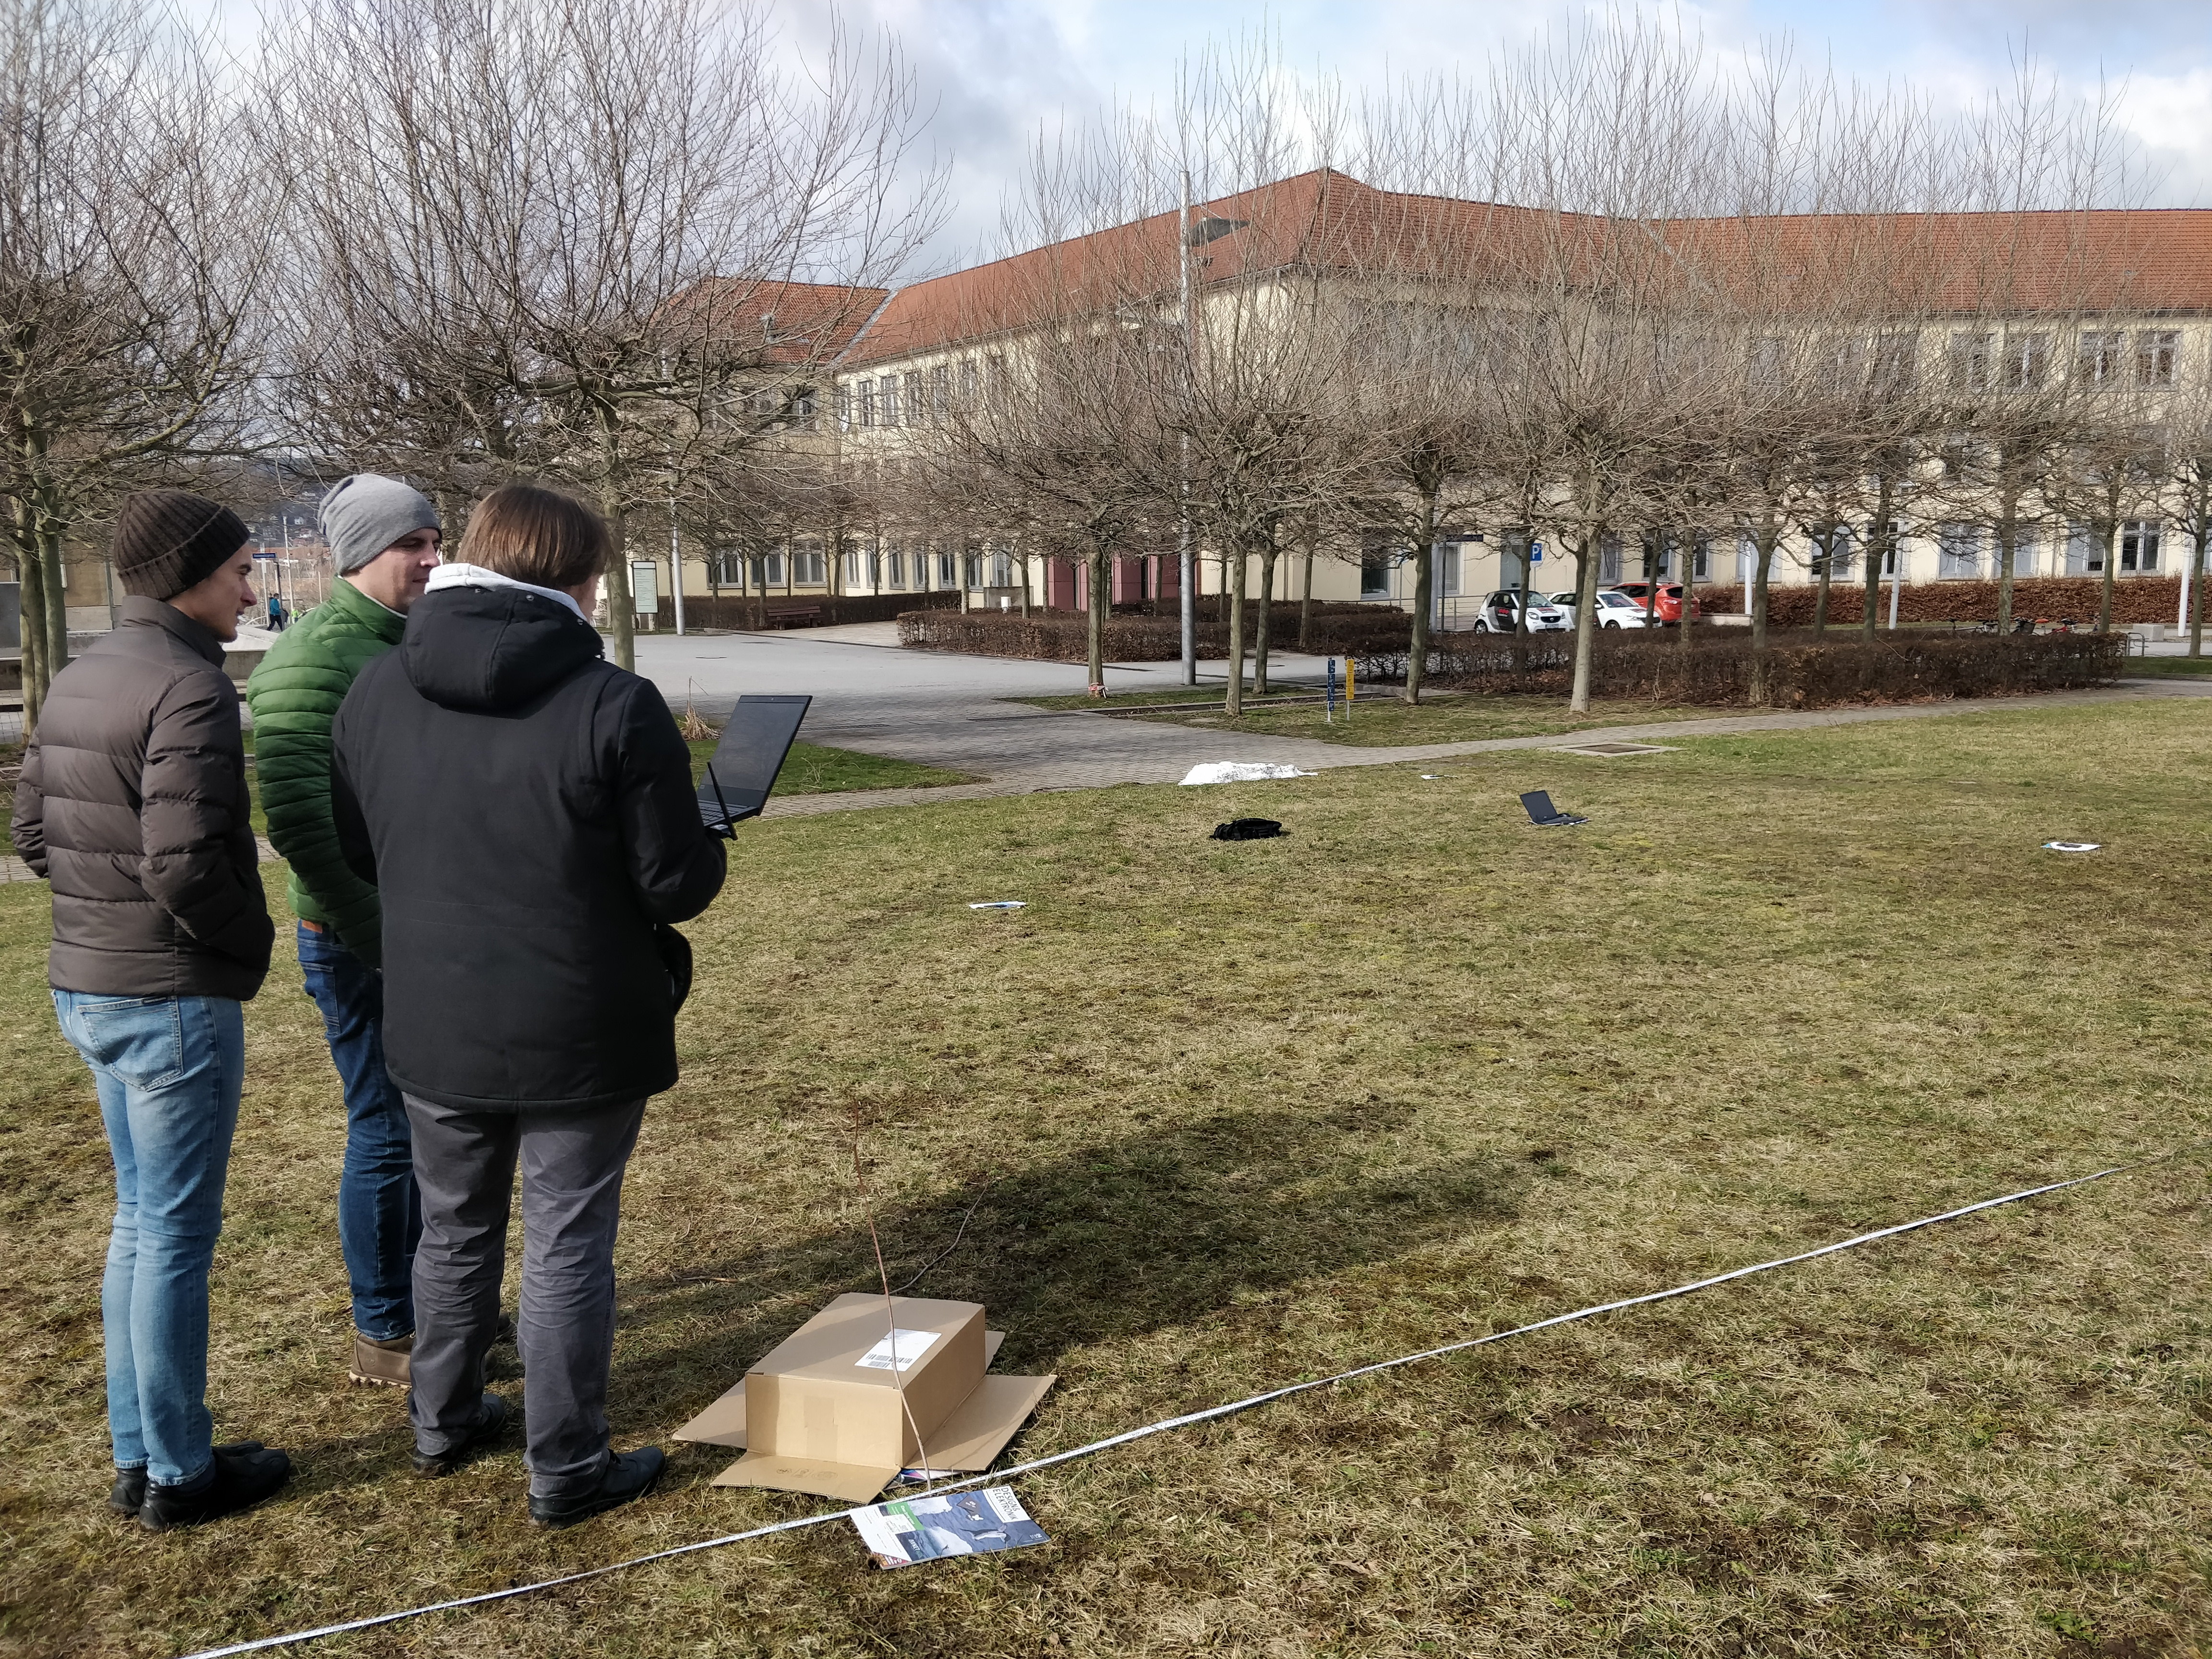
\includegraphics[width=\linewidth,keepaspectratio]{images/Layout_Problem_Discussion.jpg}
\caption{Layout Problem discussion}
\end{figure}

\subsection{Outcome}\label{outcome}

Finally, we have managed to test the framework and estimate an optimized
position for UAVs which were represented by WiFi access points. The
results showed that the framework, as well as optimization algorithms,
should be redesigned and evaluated on updated data.
